\documentclass[a4paper,12pt]{scrartcl}
\usepackage[utf8]{inputenc}
\usepackage[T1]{fontenc}
\usepackage[english,ngerman]{babel}
\usepackage{graphicx}
\usepackage{caption}
\usepackage{amsmath}
\usepackage{lmodern}
\usepackage{textcomp}
\usepackage[hidelinks]{hyperref}

\selectlanguage{german}

\hyphenation{di-gi-tal vi-su-ali-sie-ren}

%Seitenabstände
\usepackage[top=2.5cm, bottom=2.0cm, left=2.5cm, right=2.5cm]{geometry}

\title{{\fontsize{30}{20}\selectfont Satellite Computation}}
\subtitle{Jugend Forscht 2017}

\author{ Emile Hansmaennel \texttt{ emile.hansmaennel@gmail.com }}
\date{\today}

\setlength{\footskip}{30pt}

\begin{document}
 
 \maketitle 
 
 \begin{figure}[h]
  \centering
  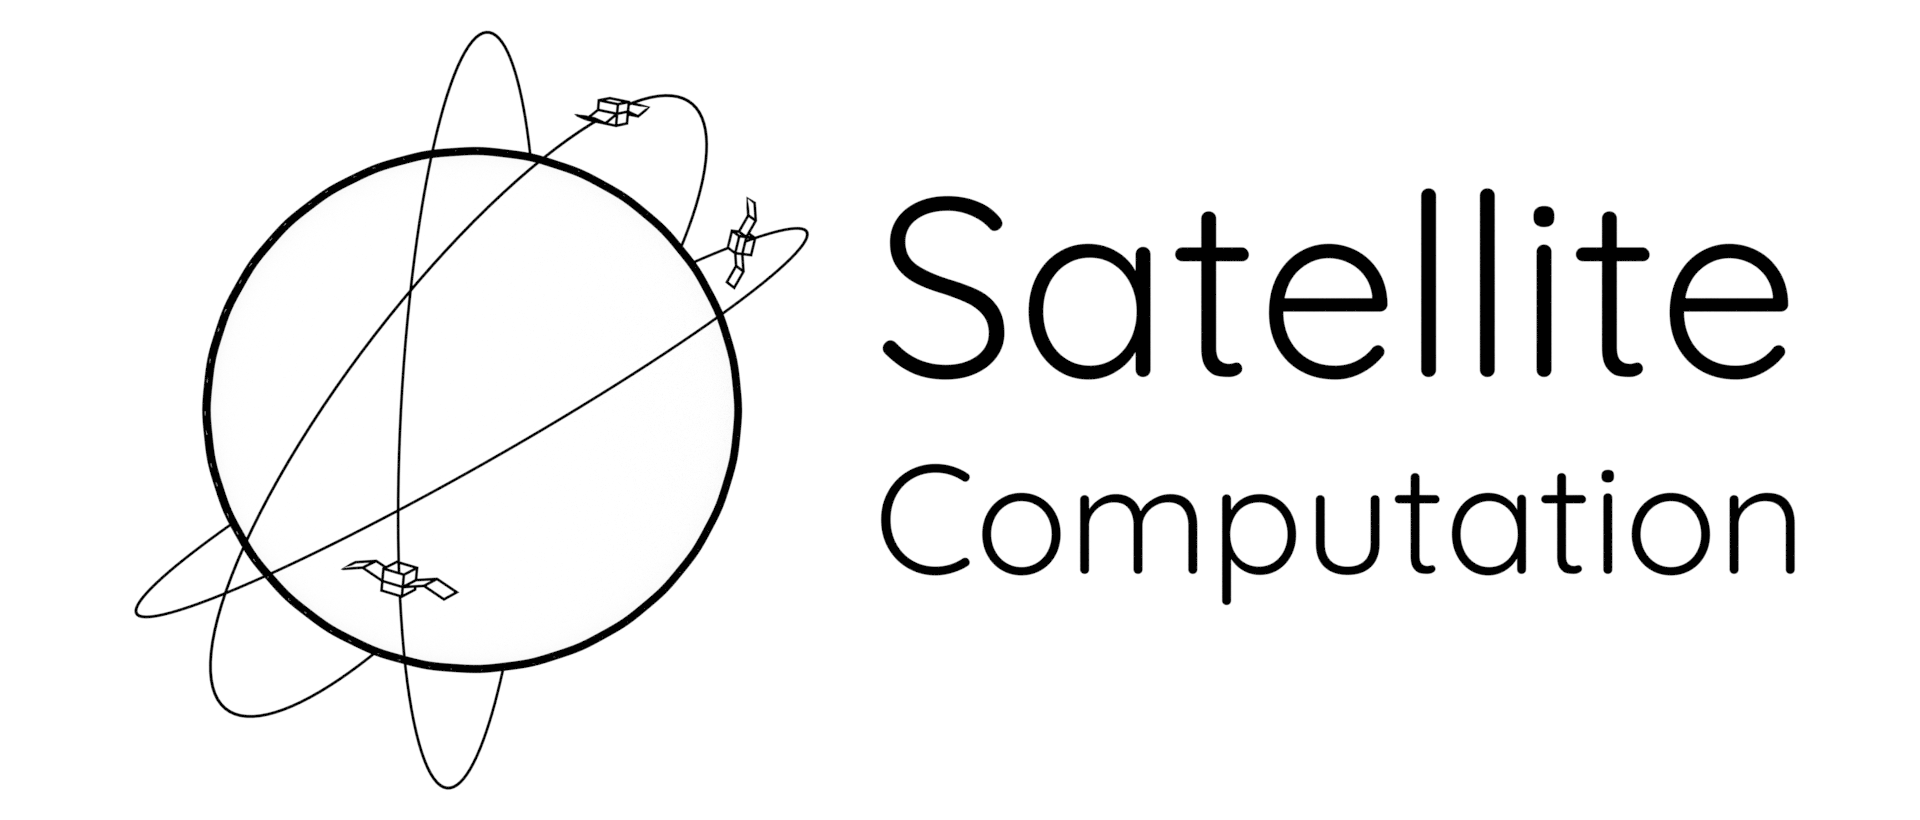
\includegraphics[width=120mm]{figs/logo5}
  \captionsetup{labelformat=empty}
  \caption{}
 \end{figure}
 
 \begin{abstract}

In dem Projekt Satellite Computation geht es darum, ein Programm zu erstellen, welches die Bahn von Satelliten Simulieren und anhand Reeler Daten eine eventuelle Kollision zwischen zwei Satelliten vorhersagen kann.

Dies wird immer wichtiger, denn die Anzahl der Satelliten in der Erdumlaufbahn steigt immer weiter und somit auch die Gefahr, dass zwei Satelliten zusammenstoßen.
Bei einer Kollision zweier Satelliten würden die Trümmerteile im schlimmsten Fall andere Satelliten treffen eine Kettenreaktion ins laufen bringen welche fatale Folgen hätte.

\end{abstract} 

 
 \thispagestyle{empty}
 \clearpage
 \newpage
 \setcounter{page}{1}
 
 \tableofcontents
 \newpage
 
 \section{Einleitung} \label{Einleitung}
 Die Bahn eines Satelliten zu berechnen, diese zu visualisieren und anschließend eine eventuelle
Kollision mit einem anderem Satelliten zu erschließen war der anfängliche Plan.
Um ein Programm herzustellen, das zu all diesem imstande ist, gibt es jedoch eine Vorraussetzung:
Der jenige der das Programm erstellen will, muss eine Programmiersprache beherrschen.
\par
Diese Vorraussetzung erfüllte ich jedoch nicht, was mich jedoch nicht davon abhielt mir eine
Programmiersprache aus der Vielzahl verschiedener Möglichkeiten auszuwählen und das Projekt damit zu durchlaufen.
Meine Wahl fiel auf Python, da ich eine strukturierte Programmiersprache gesucht habe,
welche damit auch zu komplexeren Aufgaben imstande ist.
Ein weiteres Argument für Python war, dass ich die Komplexen Zusammenhänge visualisieren wollte. Ich habe mich direkt
für das 3D-Programm Blender entschieden, da ich mich in diesem Programm bereits sehr gut
auskenne, es unglaublich flexibel ist und es schon eine Python-Integration besitzt.
Somit konnte ich mithilfe von Python Blender steuern und die Bahnen der Satelliten und die
entsprechenden Satelliten einfügen. 
\par
Um die Satelliten darzustellen brachte ich Real-Daten, jedoch wusste ich
nicht woher ich diese bekommen sollte. Nach einer intensiven Internet-Recherche fand ich eine
Quelle, welche die Daten aller Satelliten im Orbit im sogenanntem Two-Line-Element (dt. Zwei Zeilen Element) Format anbot:
(http://celestrak.com/).
\par
Mit der Zeit kamen aber auch weitere Probleme hinzu, welche sich nicht so einfach lösen ließen und es
mussten Umwege und Alternativwege genutzt werden, um an das Ziel zu kommen, welches ich mit
Freude am Ende erreichte.




 \newpage
 
 \section{Berechnung der Satelliten-Positionen, deren Bahnen und potentielle Kollisionen in der Zukunft} \label{Hauptteil}
 \subsection{Das TLE} \label{Das TLE}
Um die Bahn der Satelliten zu berechnen, diese zu visualisieren und eine mögliche Kollision zu 
erkennen, brauchte ich vor allem eines: Daten.
Diese entnahm ich wie schon erwähnt der Webseite http://celestrak.com/ welche die Informationen in 36
verschiedenen Kategorien im Two-Line-Element Format zur Verfügung stellt. Die Satelliten in einer Kategorie
sind z.B. für das Mobilfunknetz zuständig\footnote{Die sogenannten Iridium Satelliten},
eine andere Kategorie beinhaltet alle GPS-Satelliten.
\par

Das TLE Format (dt. Zwei-Zeilen-Element) indem die Bahn-Daten der Satelliten gespeichert sind, ist
wie folgt aufgebaut:

\begin{verbatim}
  ISS (ZARYA)             
  1 25544U 98067A   17013.60985296  .00002762  00000-0  49090-4 0  9990
  2 25544  51.6436  88.8992 0007382  79.8867  70.6785 15.54061452 37710
 
  123456789012345678901234567890123456789012345678901234567890123456789
         1         2         3         4         5         6         7
\end{verbatim}

\bigskip

Das TLE besteht aus zwei Zeilen in denen z.B. die Erste Ziffer für die
Zeilennummer steht. 

Die Folgende Tabelle zeigt was die Ziffern-Blöcke in der ersten Zeile beschreiben:

\bigskip
  
\begin{tabular}{l|l}
 Ziffernblock & Beschreibung: \\\hline
 & \\
 1 & Zeilennummer \\[0,1cm]
 3-7 & Satelliten Katalog Nummer \\[0,1cm]
 8 & Klassifizierung \\[0,1cm]
 10-17 & Internationale Bezeichnung \\[0,1cm]
 19-20 & Jahr \\[0,1cm]
 21-32 & Tag (Tag Nr. 40 = 9.Februar) \\[0,1cm]
 25-32 & Tagesbruchteil \\[0,1cm]
 34-43 & Wiederstandskoeffizient im SPG-Modell \\[0,1cm]
 45-52 & Vernachlässigbarer Wiederstandskoeffizient im SGP-Modell\\[0,1cm]
 54-61 & Wiederstandskoeffizient im SPG4-Modell \\[0,1cm]
 63 & Ephemeridentyp \\[0,1cm]
 65-68 & laufende Datensatz-Nummer \\[0,1cm]
 69 & Prüfsumme Modulo 10 \\[0,1cm]
 
\end{tabular}

\bigskip

In meinem Fall war der Ziffernblock 19-32 von Bedeutung, denn ausgewertet hat er mir die Zeit
gegeben, an dem die jeweiligen Werte aufgenommen wurden. Dies war wichtig um nicht aus versehen
mit alten Werten weiterzuarbeiten, was im Echtfall zu fatalen Folgen geführt hätte.
Das SGP-Modell (Simplified General Perturbation model) sind Modelle zur Berechnung der sogennanten Orbitalszustandsvektoren.

Die Folgende Tabelle beschreibt die zweite Zeile:

\bigskip
  
\begin{tabular}{l|l}
 Ziffernblock & Beschreibung: \\\hline
 & \\
 1 & Zeilennummer \\[0,1cm]
 3-7 & Satelliten Catalog Nummer \\[0,1cm]
 9-16 & Inklination \\[0,1cm]
 18-25 & Rektazension des aufsteigenden Knotens \\[0,1cm]
 27-33 & Numerische Exzentrizität \\[0,1cm]
 35-42 & Argument des Perigäums \\[0,1cm]
 44-51 & Mittlere Anomalie \\[0,1cm]
 53-63 & Mittlere Bewegung \\[0,1cm]
 64-68 & Umlauf Nr. \\[0,1cm]
 69 & Prüfsumme Modulo 10 \\[0,1cm]
\end{tabular}

\bigskip

Die zweite Zeile beinhaltet eine Menge wichtiger Werte:
Die Inklination, die Rektazension des Aufsteigenden Knotens, die numerische Exzentrizität der
Umlaufbahn, das Argument des Perigäums, die Mittlere Anomalie, die Mittlere Bewegung, und die
Anzahl der Umläufe seit dem Start.
Diese Informationen geben Aufschluss wo sich der Satellit im Verhältnis zu der Erde und deren Koordinatensystem befindet.
\par

\subsection{Die Achsen in Blender}

\begin{figure}[h]
 \centerline{
 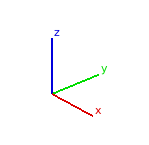
\includegraphics[height=0.5\textwidth]{figs/Achsen_w}
 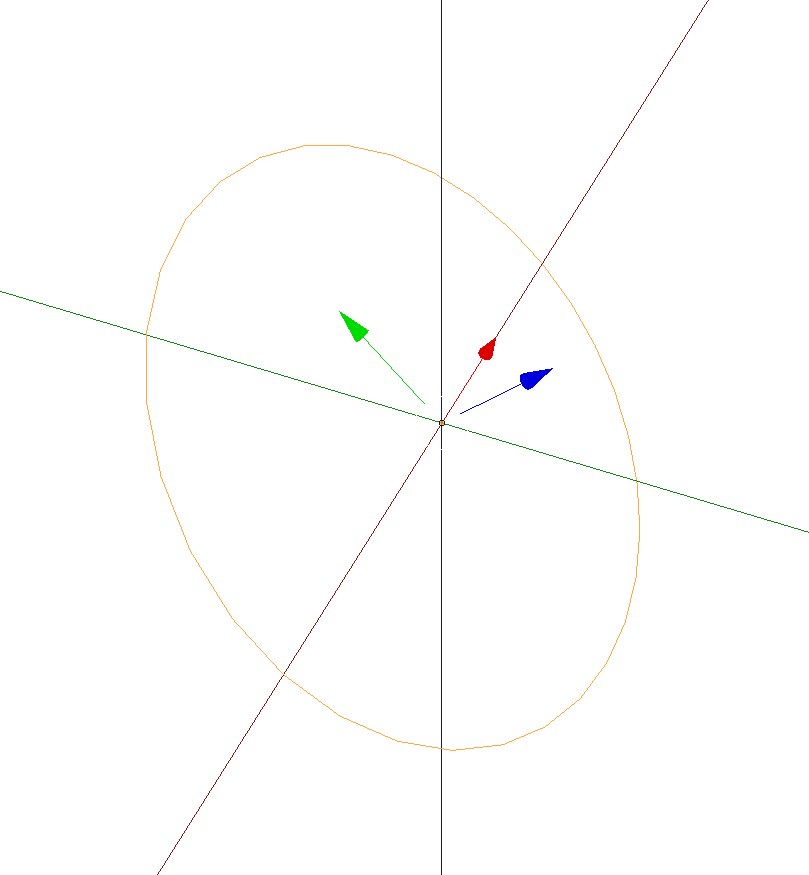
\includegraphics[height=0.5\textwidth]{figs/LokaleAchsen_w}
 }
 \caption{Die Achsen in Blender \newline Links die Globale Achsen, Rechts die Lokale Achsen eines Kreises}
 \label{fig:Achsen}
\end{figure}

Um im 3-Dimensionalen Raum Objekte wie in meinem Fall eine Bahn Ellipse zu rotieren, muss
festgelegt sein in welche Richtung rotiert wird. Es gibt zwei Möglichkeiten: Entweder das Objekt wird um eine
globale Achse gedreht, sprich egal wie das Objekt schon gedreht ist, es wird immer wieder um eine
festgelegte Achse gedreht oder das Objekt wird um eine lokale Achse gedreht, wobei wie in der
rechten Abbildung dargestellt, die Achsen sich sozusagen mitdrehen.

\subsection{Die Verwendung der Daten}

Die Daten aus dem TLE definieren die Lage der Bahn-Ellipse im Raum.
In meinem Programm habe ich diese Daten genutzt und wie folgt eingebaut:
\par
Hier der Ablauf des Programms in Worte gefasst:
\par
Als erstes muss ein Kreis beschrieben werden, der mithilfe von Python in Blender eingefügt wird.
Um aus dem Kreis eine Ellipse zu bekommen, muss
der Kreis um einen bestimmten Faktor gestreckt werden. Dieser Faktor lässt sich mithilfe der
Werte aus dem TLE berechnen:
\par

\begin{equation} \label{eq:semimajoraxis}
  a = \left( \frac{6.6228}{(n_0)^\frac{2}{3}} * 6371 \right)
\end{equation}

Formel der Großen Halbachse\footnote{http://www.tuit.ut.ee/sites/default/files/tuit/arvutitehnika-thesis-msc-2014-ploom-indrek-text-20140528.pdf, s. 17, Formel (7)} (\ref{eq:semimajoraxis})

\begin{equation} \label{eq:apogee}
  \text{Apogäum} = a \cdot (1 + e_0) - 6378
\end{equation}

\begin{equation} \label{eq:perigee}
  \text{Perigäum} = a \cdot (1 - e_0) - 6378
\end{equation}


Der streckfaktor an der x-Achse (Abbildung \ref{fig:Achsen}) ist gleich der Länge des
Apogäums (\ref{eq:apogee}) wobei \( e_0 = \text{Numerische Exzentrizität} \) und 
\( n_0 = \text{Mittlere Bewegung} \) gilt. Die Streckung an der y-Achse ist gleich der Länge des
Perigäums (\ref{eq:perigee}).

Das Ergebnis ist eine Ellipse, die jedoch noch keine Inklination besitzt. Um eine
\textbf{Inklination} \( i \) zu erzeugen, muss festgelegt werden von welcher Referenz-Ebene aus die
Inklination ausgeht. Für die Inklination von Satelliten-Bahnen wurde festgelegt, dass als
Referenz-Ebene die Äquator-Ebene genommen wird (Abbildung \ref{fig:BahnelementeEllipse}). Da
die Ellipse im Ursprung des Koordinatensystems ist, kann sie einfach an der x-Achse mit dem
wert der Inklination aus dem TLE \footnote{Der Wert wird vorher noch in Bogenmaß umgewandelt}
rotiert werden um die Inklination darzustellen.
\\\par

\begin{figure}[h]
  \centering
  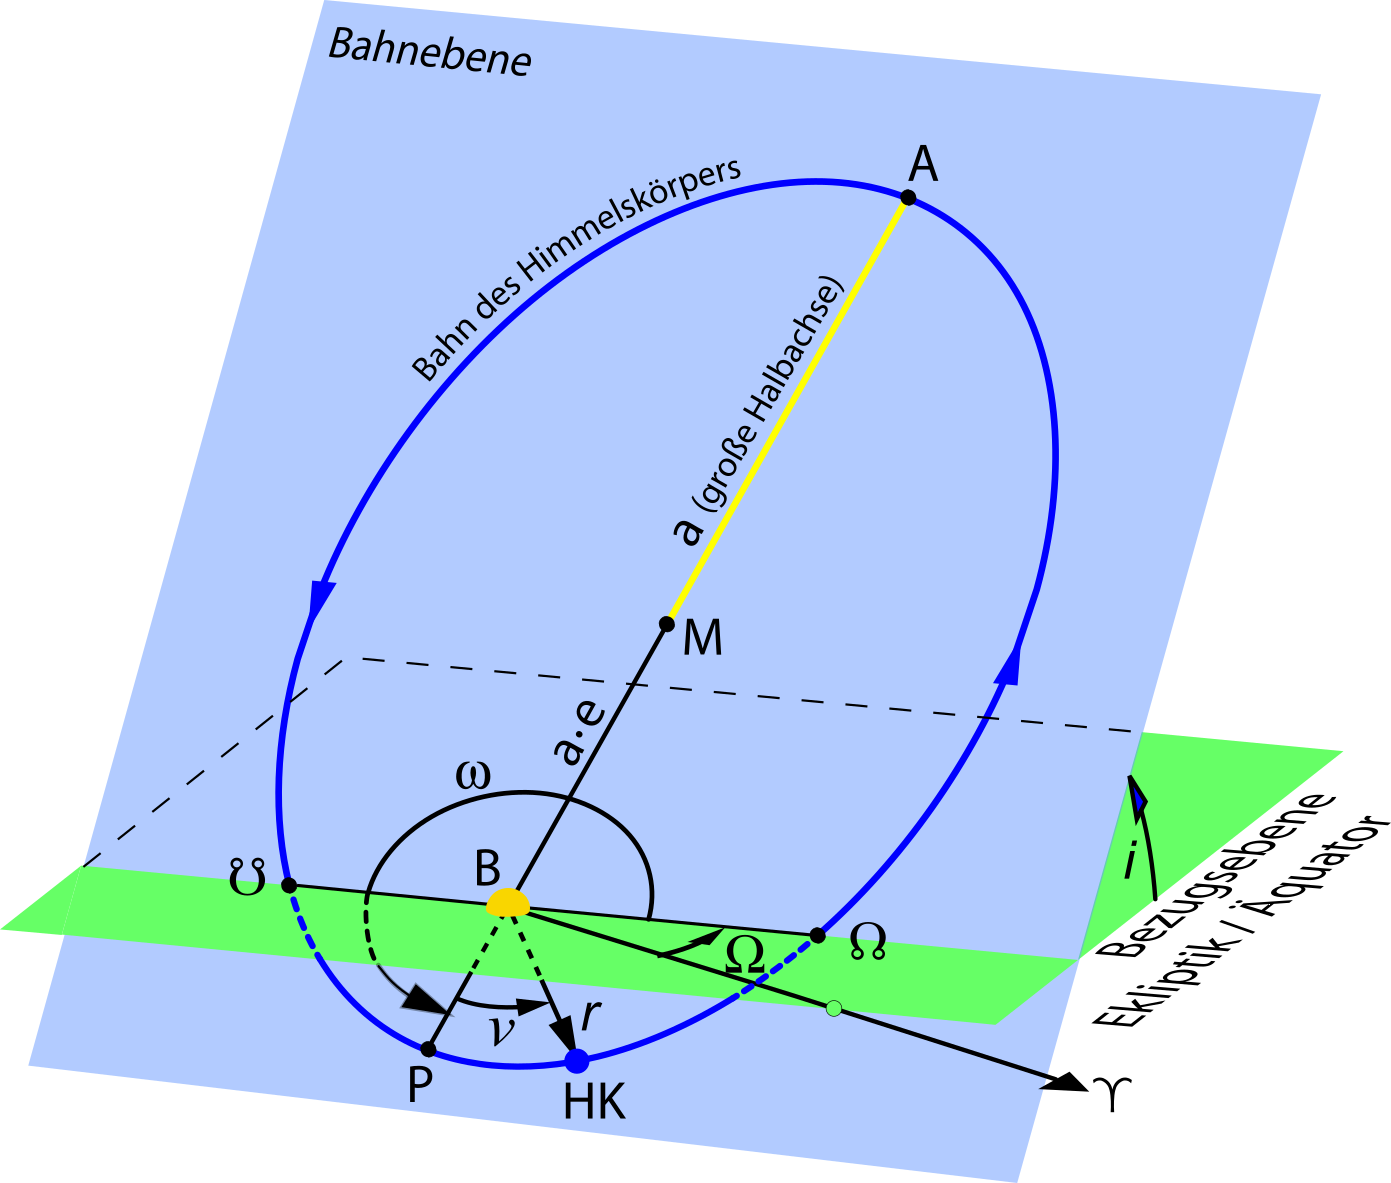
\includegraphics[width=120mm]{figs/BahnelementeEllipse}
  \captionsetup{labelformat=parens}
  \caption{Die Bahn-Elemente der Ellipse \newline Quelle: Wikipedia.org, Länge des Aufsteigenden Knotens}
  \label{fig:BahnelementeEllipse}
\end{figure}


\textbf{Die Rektazension des aufsteigenden Knotens} \( \Omega \) beschreibt die Drehung um die z-Achse
(Abbildung \ref{fig:Achsen}).
Der sogenannte aufsteigende Knoten ist der Punkt an dem die Bahn-Ellipse die Referenz-Ebene von
Süden nach Norden durchstößt. Die Rektazension des aufsteigenden Knotens beschreibt den Winkel
zwischen der Strecke vom Mittelpunkt der Ellipse zum sogenannten Frühlingspunkt.
Als Frühlingspunkt wird der Schnittpunkt des Äquators mit der Elliptik bezeichnet.
\\\par

\textbf{Das Argument der Periapsis} \( \omega \) wird dazu genutzt, die Rotation der Ellipse um
die lokale z-Achse (Abbildung \ref{fig:Achsen}, rechts) zu beschreiben. Voraussetzung für die
Anwendung des Argument des Perigäums ist, dass die Ellipse schon eine Inklination besitzt.
\\\par

\newpage
\subsection{Programm Code für Python} \label{Code}

Das erste Teil-Ziel war es, einen Wert wie z.B. den Namen eines Satelliten zu bekommen indem
im Code einfach die Funktion 

\begin{verbatim}
 TLE.get(``name'', category, satNr)
\end{verbatim}

ausgeführt wurde. Dies funktionierte einwandfrei und um z.B. den Wert der Inklination aller
Satelliten aus der Iridium-Kategorie zu bekommen und einer Liste hinzuzufügen wurde folgender
Code ausgeführt:

\begin{verbatim}
01  import TLE
02  
03  category = "iridium"
04  inc = []
05  
06  for satellite in category:
07    inc.append(TLE.get("Inclination", category, satellite)
\end{verbatim}

Die Daten konnten aus dem TLE relativ einfach abgefragt werden, sodass es schnell
möglich eine Bahn in Blender darzustellen, bei der sich der jeweilige Satellit auf
einer Kreisbahn bewegte:

\begin{verbatim}
01 import TLE
02 import bpy
03 import math
04 
05 category = "iridium"
06 inc = []
07 satNr = 1
08 
09 inc.append(TLE.get("Inclination", category, satNr) * math.pi / 180)
10 
11 bpy.ops.mesh.primitive_circle_add(radius=1, vertices=60)
12 bpy.context.object.name = "orbit"
13 bpy.object.convert(target='CURVE)
14 
15 bpy.ops.mesh.primitive_cube_add(radius=0.1)
16 bpy.context.object.name = "orbit sat"
17 
18 orbit = bpy.context.scene.objects["orbit]
19 sat = bpy.context.scene.objects["orbit sat"]
20 
21 orbit.select = False
22 sat.select = True
23 
24 sat.location[1] = 1
25
26 bpy.context.scene.objects.active = orbit
27 bpy.ops.object.parent_set(type='FOLLOW')
28 orbit.rotation_euler[0] = inc
 
\end{verbatim}

Bedeutung der Zeilen im obigen Code:
\\\bigskip

\begin{tabular}{l l}
 Zeile & Beschreibung: \\
 1-3 & Import der Modul TLE (\ref{Code}), bpy (BlenderPython) und math \\
 5 & Definition der Kategorie \\
 6 & Definition der Liste zum Speichern der Inklination \\
 7 & Definition der Nummer des Satelliten aus der Kategorie \\
 9 & Hinzufügen des Wertes der Inklination in Grad zur Liste inc \\
 11 & Einfügen eines 60-eckes in Blender mit dem Radius 1 \\
 12 & Umbenennung des Kreises zu ``orbit'' \\
 13 & Konvertierung des Kreises zu einer Kurve \\
 15 & Einfügen eines Würfels, welcher den Satelliten darstellt \\
 16 & Umbenennen des Satelliten zu ``sat'' \\
 18-19 & Definition von ``orbit'' und ``sat'' zur einfachen Auswahl \\
 21 & Abwählen der Satelliten-Bahn \\
 22 & Auswählen des Satelliten \\
 24 & Verschieben des Satelliten zu x = 1 \\
 26 & Die Satelliten-Bahn als aktives Objekt markieren \\ 
 27 & Den Satelliten an die Satelliten-Bahn mit dem Attribut 'FOLLOW' anhängen \\
 28 & Die Satelliten-Bahn um den Wert inc an der x-Achse neigen \\
 
 
\end{tabular}
\bigskip

Die in Blender dargestellte Bahn war jedoch in vieler Hinsicht nicht genau: Es fehlte noch die
Einbringung mehrerer Werte: die Rektazension des aufsteigenden Knotens, das Argument des
Perigäums, der Apogäums / Perigäums und die Umlauf-Geschwindigkeit.
\par
Nachdem ich diese Werte einbezogen hatte, konnte ich eine reelle Satelliten-Bahn in Blender erzeugen.
Doch was mich störte war, dass ich ja nur einen Satelliten angezeigt bekam und die mögliche
Kollision eines Satelliten mit einem anderem vorhersagen wollte wozu ich mehrere Satelliten
bräuchte. 

\begin{figure}[h]
  \centering
  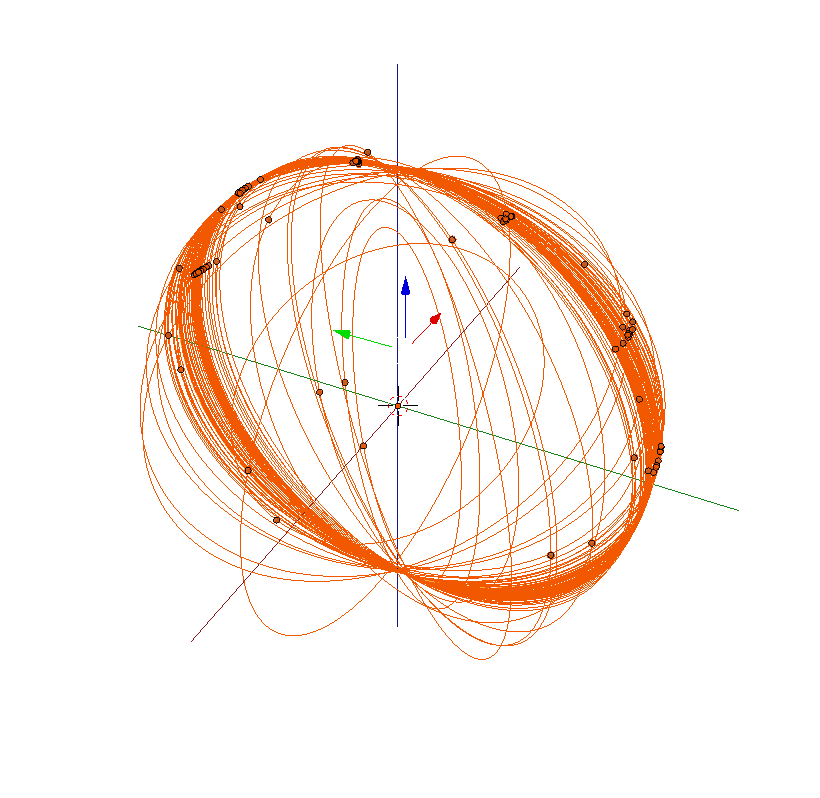
\includegraphics[height=0.5\textwidth]{figs/iridium_sat_all_w}
  \caption{Die gesamten Iridium Satelliten in Blender Visualisiert}
  \label{fig:iridium_sat_all}
\end{figure}

Also steckte ich
meinen Code in eine Schleife, änderte ihn leicht ab und bekam die Bahn aller Satelliten in einer
Kategorie angezeigt (Abbildung \ref{fig:iridium_sat_all}).
\par

\subsection{Vom 3-Dimensionalen ins 2-Dimensionale zu Kollisionen}

Das nächste Ziel war es, eine mögliche Kollision vorherzusagen. Eine Kollision ist dann geschehen,
wenn zwei Objekte zu selben Zeit am selben Ort sind oder zur selben Zeit sehr nah aneinander sind.
Eine Voraussetzung, um die Kollision zweier Objekte zu bestimmen, ist die Position der Objekte zu
einer bestimmten Zeit zu kennen. Problematisch war, dass als ich mithilfe von Python die Position
der Satelliten abfragen wollte, ein Fehler bekam: Da der Satellit an der Bahn hing, war ein
auslesen der Position nicht möglich. Die löste ich indem ich den Satelliten erst von der Bahn
``abkoppelte'', die Position aus las und ihn wieder ``ankoppelte''. Dies funktionierte wunderbar.
Die ausgelesenen Werte speicherte ich in einer Liste die ich im Anschluss in einem
Koordinatensystem ausgab.

\begin{figure}[h]
 \centerline{
 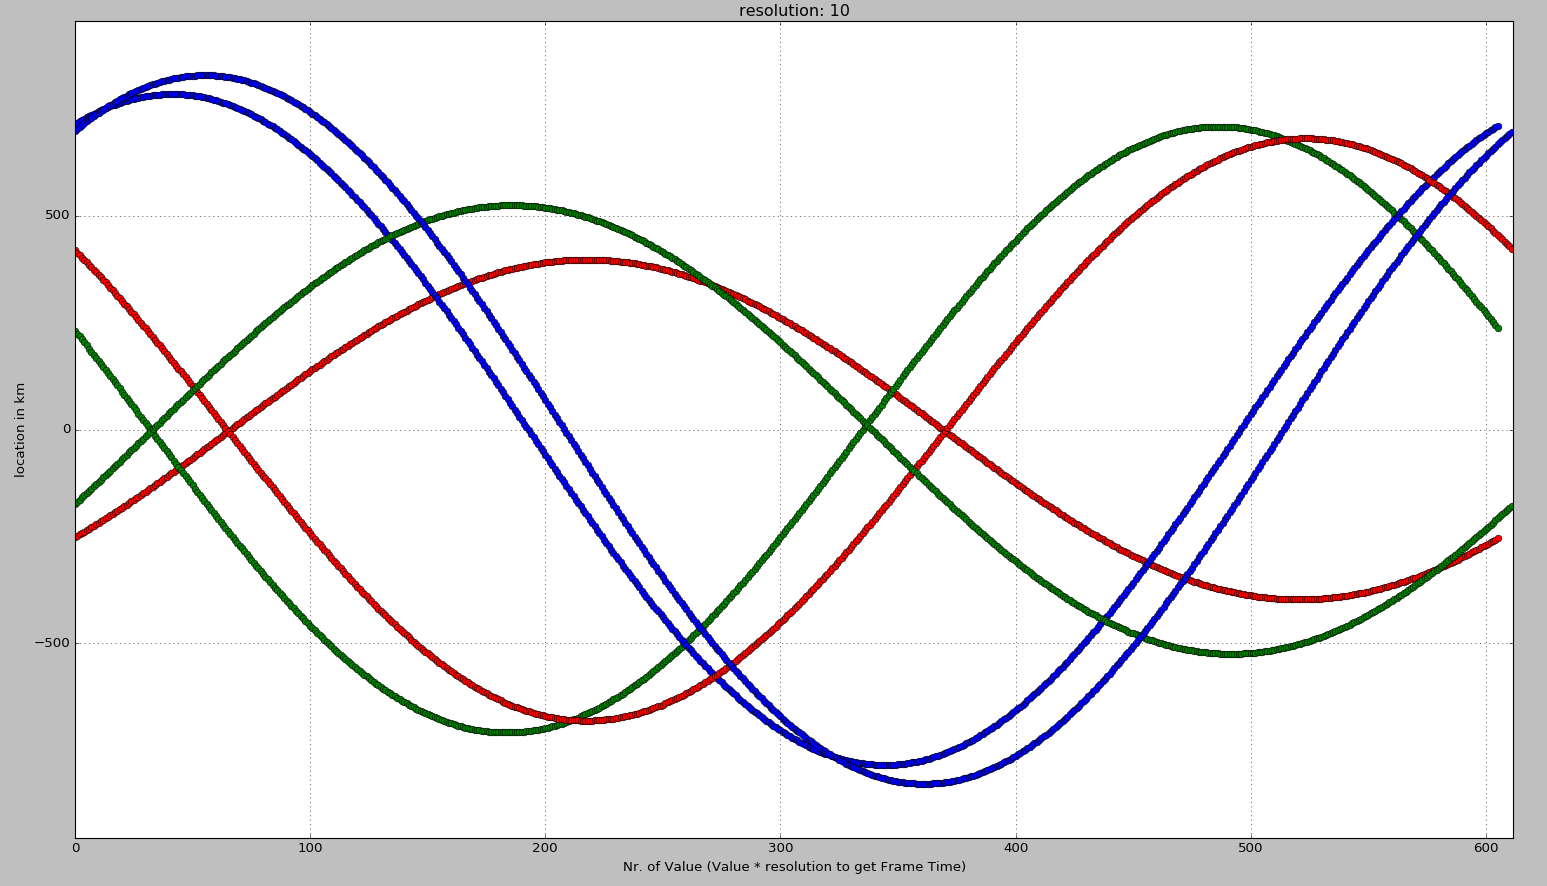
\includegraphics[width=0.5\textwidth]{figs/argos_2sat_2D}
 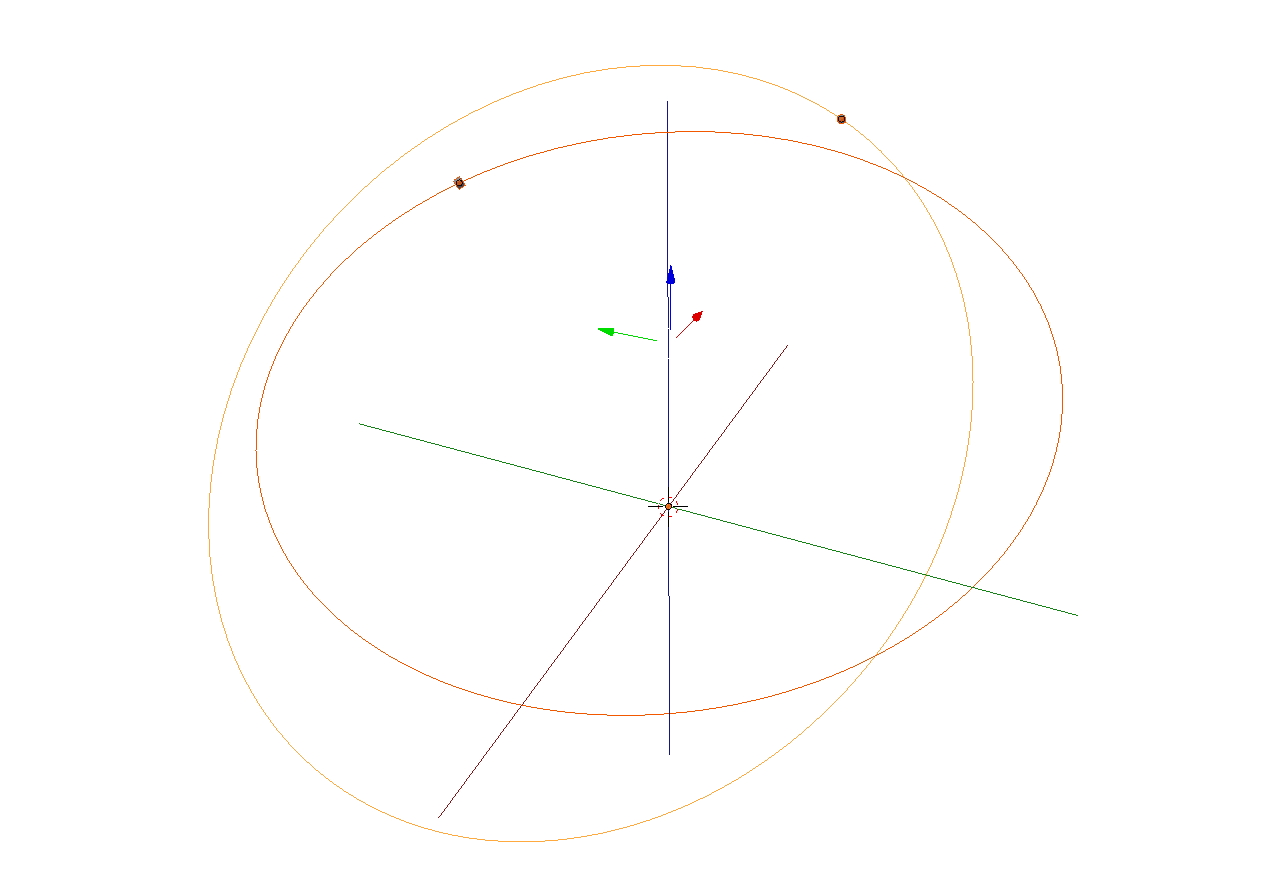
\includegraphics[width=0.5\textwidth]{figs/argos_2sat_3D_w}
 }
 \caption{Beispiel der Graphen anhand von zwei Satelliten}
 \label{fig:argos_2sat}
\end{figure}

\begin{figure}[h]
 \centerline{
 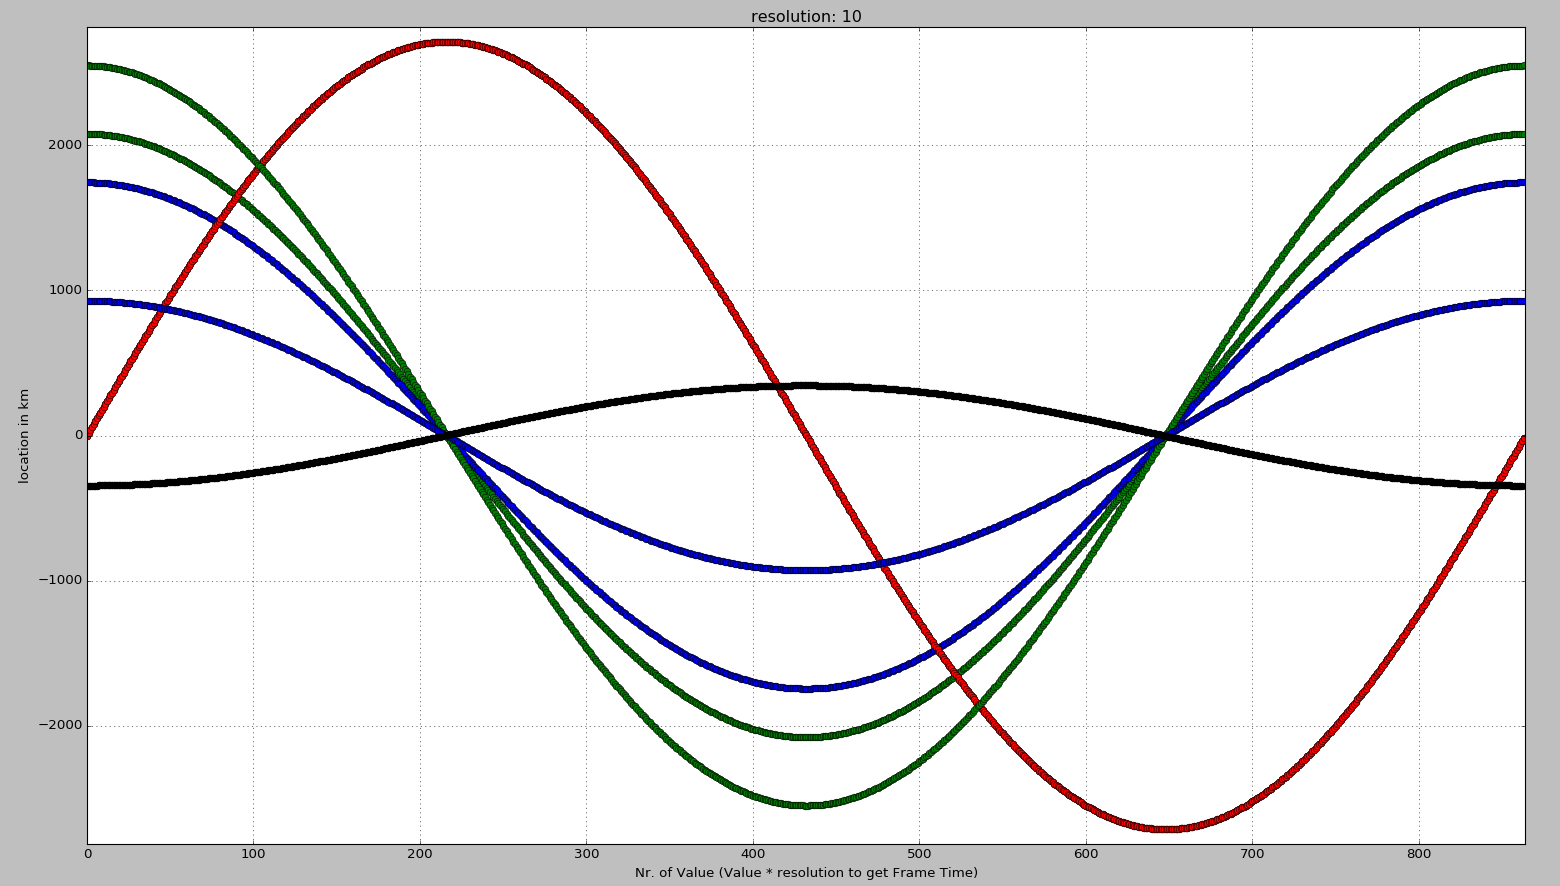
\includegraphics[width=0.5\textwidth]{figs/dummy_2sat_2D}
 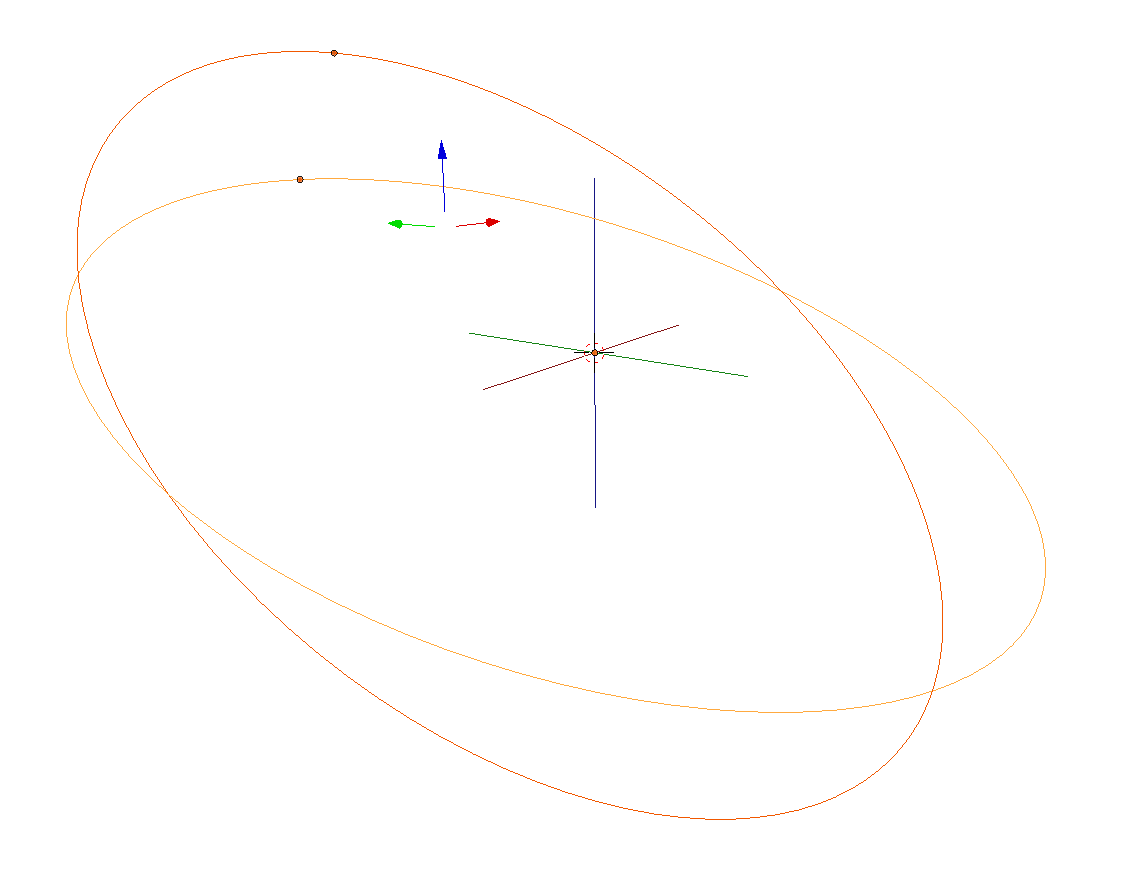
\includegraphics[width=0.5\textwidth]{figs/dummy_2sat_3D_w}
 }
 \caption{Beispiel einer Kollision (Daten künstlich hergestellt) \newline Es ist nur eine x-Achse (Rot) sichtbar, da die x-Position der Beiden Satelliten die ganze Zeit identisch ist}
 \label{fig:dummy_2sat}
\end{figure}

In Abbildung \ref{fig:argos_2sat} ist links ein Koordinatensystem mit den Bahnen von zwei
Satelliten aus der sogenannten ``argos''-Kategorie abgebildet, rechts sind die entsprechenden
Bahnen im 3-Dimensionalen Raum zu sehen. Würde eine Kollision vorliegen, würden die jeweiligen
Bahnen sich an einem Punkt zur gleichen Zeit kreuzen).
\par
Als Beispiel einer Kollision kann Abbildung \ref{fig:dummy_2sat} genommen werden, welche aus zwei
künstlichen TLEs entstand. Da eine Kollision vorhanden ist, wenn zu einem Zeitpunkt
\( x_1 - x_2 \approx 0 \; \vee \; y_1 - y_2 \approx 0 \; \vee \; z_1 - z_2 \approx 0\) erfüllt ist,
kollidieren in diesem Beispiel die Satelliten.
(Es ist nur ein roter Graph sichtbar, da die x-Werte über die ganze Zeit hinweg identisch sind).
Der schwarze Graph beschreibt für jeden Zeitpunkt die Summe der Differenz der Position der
jeweiligen Satelliten.

\begin{figure}[h]
 \centerline{
 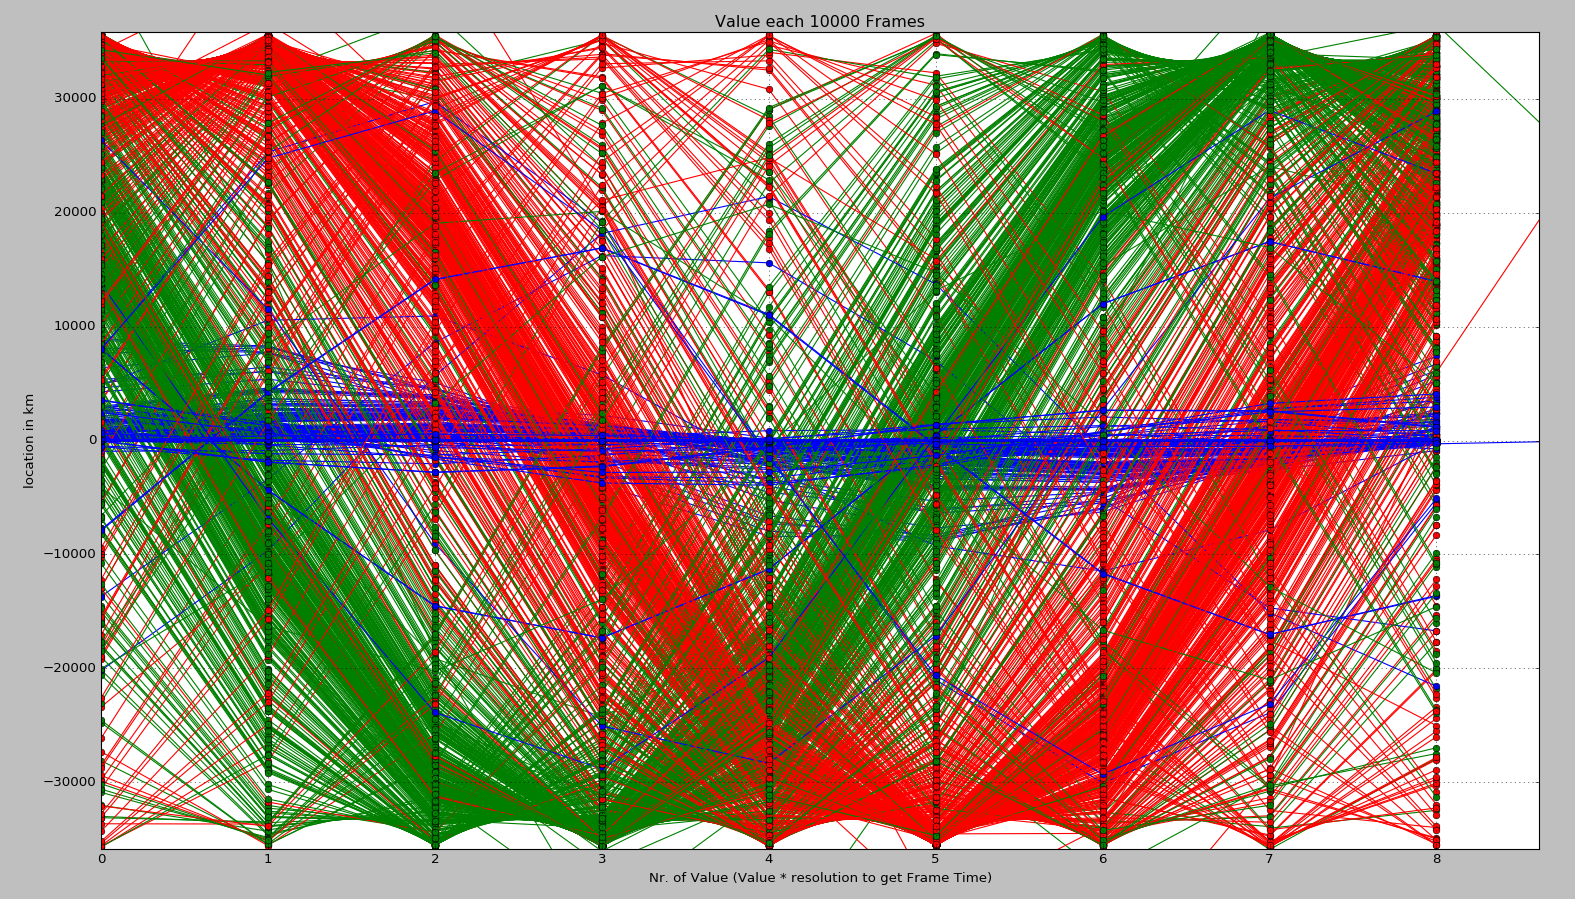
\includegraphics[width=0.5\textwidth]{figs/geo_allsat_2D}
 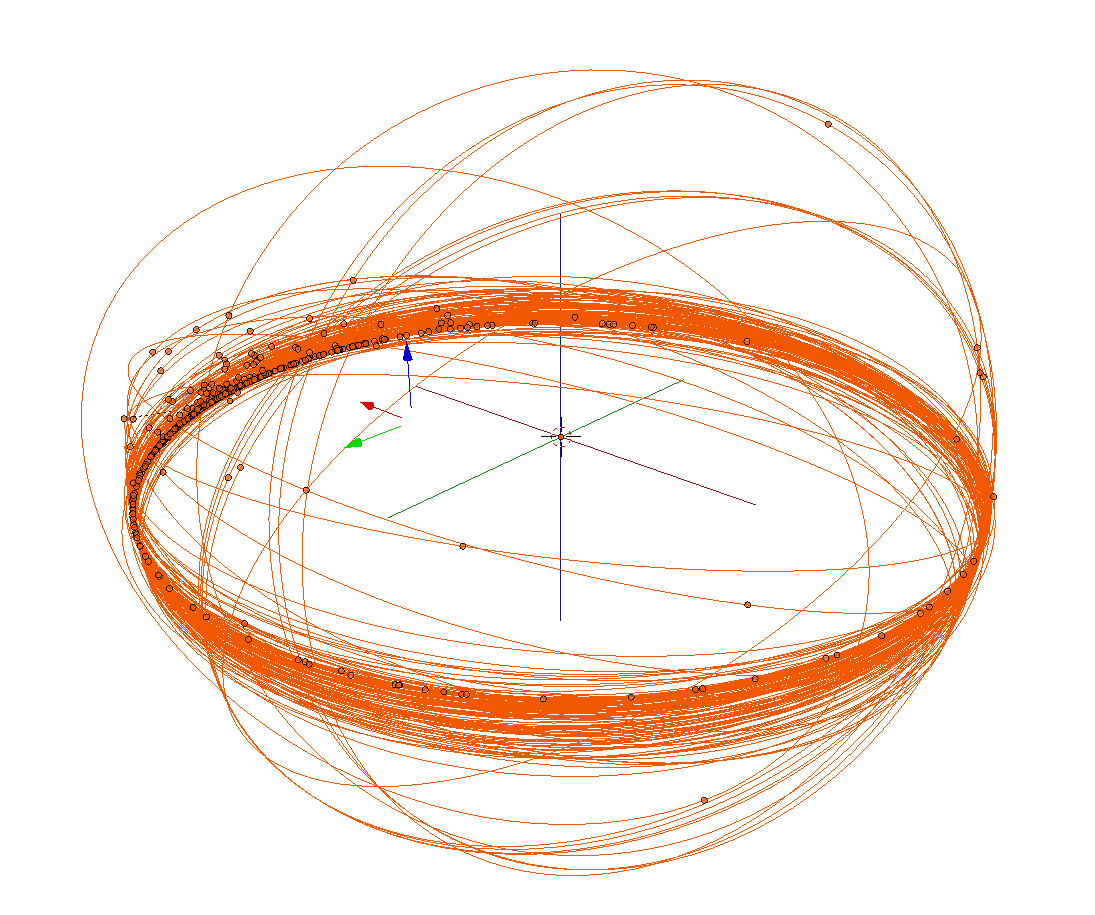
\includegraphics[width=0.5\textwidth]{figs/geo_allsat_3D_w}
 }
 \caption{Alle geostationären Satelliten in einem Koordinatensystem}
 \label{fig:geo_allsat}
\end{figure}

\bigskip

Problematisch wird diese Methode, wenn wie in Abbildung \ref{fig:geo_allsat} (links) sehr viele Satelliten
auf eine mögliche Kollision überprüft werden sollen. Theoretisch muss zu jedem Zeitpunkt die
Entfernung zwischen allen Satelliten berechnet werden. Die unten stehende Tabelle verdeutlicht
dieses Prinzip. Genau genommen müssen nicht alle Felder berechnet werden: die Entfernung zwischen
einem Satelliten und dem selben Satelliten ist immer 0 und die Werte im unterem Teil der
Tabelle brauchen nicht ausgerechnet zu werden, da sie schon oben stehen \footnote{Das Ergebniss der jeweiligen Rechnungen wird als Absoluter Wert genommen}. 

\bigskip

\begin{tabular}{l | l | l | l | l}
  & sat[1][x][t] & sat[2][x][t] & sat[3][x][t] &  \\
  & sat[1][y][t] & sat[2][y][t] & sat[3][y][t] & ... \\
  & sat[1][z][t] & sat[2][z][t] & sat[3][z][t] &  \\\hline
 
 sat[1][x][t] &  & sat[2][x][t] - sat[1][x][t] = 0 & sat[3][x][t] - sat[1][x][t] \(\neq\) 0 &  \\
 sat[1][y][t] &  & sat[2][y][t] - sat[1][y][t] = 0 & sat[3][y][t] - sat[1][y][t] \(\neq\) 0 & ... \\
 sat[1][z][t] &  & sat[2][z][t] - sat[1][z][t] = 0 & sat[3][z][t] - sat[1][z][t] \(\neq\) 0 &  \\\hline
 
 sat[2][x][t] &  &  & sat[3][x][t] - sat[2][x][t] \(\neq\) 0 &  \\
 sat[2][y][t] &  &  & sat[3][y][t] - sat[2][y][t] \(\neq\) 0 & ... \\
 sat[2][z][t] &  &  & sat[3][z][t] - sat[2][z][t] \(\neq\) 0 &  \\\hline
 
 sat[3][x][t] &  &  &  &  \\
 sat[3][y][t] &  &  &  & ... \\
 sat[3][z][t] &  &  &  &  \\\hline
 
 ... & ... & ... & ... & ...
\end{tabular}

\bigskip

Wenn die Summe der Werte in einem Feld der Tabelle gleich 0 ist, kann davon ausgegangen werden, dass der
entsprechende Satellit in der Zeile mit dem Satelliten aus der Spalte kollidiert ist.
\par
Die Folgende Tabelle zeigt ein Beispiel:

\bigskip

\begin{tabular}{l | l | l | l}
               & \(x_1=\) -2711  & \(x_2=\) -2711   & \\
               & \(y_1=\) -18    & \(y_2=\) -15     & ... \\
               & \(z_1=\) -6     & \(z_2=\) -12     & \\\hline
 
\(x_1=\) -2711 &                 & 2711 - 2711 = 0  & \\
\(x_1=\) -18   &                 & 18 - 15 = 3      & ...\\
\(x_1=\) -6    &                 & 6 - 12 = 6       & \\
               &                 & \(\sqrt[2]{0^2 + 3^2 + 6^2} \approx 6.708\) & \\\hline
 
\(x_2=\) -2711 & 2711 - 2711 = 0 &                  & \\
\(y_2=\) -15   & 15 - 18 = 3     &                  & ... \\
\(z_2=\) -12   & 12 - 6 = 6      &                  & \\
               & \(\sqrt[2]{0^2 + 3^2 + 6^2} \approx 6.708\)  &                  & \\\hline
           ... & ...             & ...              & ... 
\end{tabular}

\bigskip

\begin{equation}\label{eq:pythargoras3D}
 \text{Abstand der Satelliten} = \sqrt[2]{(x_1 - x_2)^2 + (y_1 - y_2)^2 + (z_1 - z_2)^2}
\end{equation}

\bigskip

Zu sehen ist, wie die Positionswerte der beiden Satelliten verrechnet werden und am Ende der 
Satz des Pythargoras für den 3-Dimensionalen Raum(\ref{eq:pythargoras3D}) angewendet wird:



Dies bedeutet die beiden Satelliten kollidieren \textbf{nicht}, fliegen jedoch eng aneinander vorbei.
 \newpage
 
 \section{Ergebnisse} \label{ergebnisse}
 Das Ergebniss des Projektes ist erfreulich: Es ist möglich mithilfe des Python Programmes die
Satellitenbahnen aller Satelliten in Blender mithilfe der TLEs aus dem Internet darzustellen,
sowohl 2-dimensional als auch 3-dimensional. Die Vorhersage von eventuellen Kollisionen ist
ebenfalls möglich.
\par
Das Programm kann in der Zukunft erweitert werden, sodass Störfaktoren wie z.B die
Anziehungskraft des Mondes in den Berechnungen berücksichtigt werden können.
 \newpage
 
 \section{Quellen und Hilfen} \label{quellen}
 \begin{center}
 \textbf{
  Das Python-Programm sowie die Blender Darstellungen wurden vollständig ohne fremde Hilfe selber erstellt.
 }
\end{center}
\par Einen Großteil der Formeln fand ich durch eine Wikipedia Recherche, jedoch wurden auch Informationen aus dem 'SPACETRACK REPORT' von Felix R. Hoots und Ronald L. Roerich,
No. 3 (Dec. 1980) entnommen. 
\par Das Programieren in der Programiersprache Python habe ich wärend des Projektes mithilfe der Python-Documentation gelernt. Mit dem Umgang des 3D-Programms Blender
bin ich schon vertraut gewesen. Die Grundlagen für \LaTeX, in dem diese Langfassung geschrieben wurde, erlernte ich durch das Studieren diverser Beiträge in Foren und der Einsicht
in das Jugend Forscht Projekt von Konstantin Bosbach, Tilman Hoffbauer und Steffen Ritsche aus dem vorherigem Jahr (2016, Underwater Accoustic Communication).
\par Da es das erste Mal war, dass ich Python mit Blender kombiniert habe, musste ich mich in diesen Bereich ebenfalls einarbeiten.
Dabei war die Blender API Documentation (www.blender.org/api) von großer Hilfe.


\raggedleft
\section*{Dank gilt...} 
\paragraph{Herrn Jörg Thar} meinem Betreuer

\centering
\vspace{0.5cm} \textbf{Außerdem gilt mein Dank allen, die mich auf jede nur erdenkliche Weise unterstützt haben.}
 
\end{document}
